\section{The Unified Field Equation (UFE)}
%=============================================================================

%-----------------------------------------------------------------------------
\subsection{Torsionful Geometric Action}
%-----------------------------------------------------------------------------

\begin{definition}{UFE Action}{UFEaction}
On a manifold $M^{4+n}$ with metric $\hat{g}_{AB}$ and torsionful connection 
$\hat{\Gamma}^A_{BC}$, the action is:
\begin{equation}
    S = \int d^{4+n}x\sqrt{-\hat{g}}\left[
        \frac{1}{2\hat{\kappa}^2}\hat{R}(\hat{\Gamma}) 
        + \mathcal{L}_{\text{tors}}(K,T) 
        - \frac{1}{4}F_{AB}F^{AB}
        + \frac{1}{2}\hat{g}^{AB}\partial_A a\,\partial_B a 
        - V(a) 
        + \cthree\, a\, F_{AB}\tilde{F}^{AB}
    \right]
\end{equation}
Here $\hat{R}(\hat{\Gamma})$ denotes the Ricci scalar constructed from the full torsionful connection $\hat{\Gamma}$.
\end{definition}

\noindent\textbf{Maxwell convention.} We treat the U(1) gauge potential $A$ as a one-form and define the field strength by the exterior derivative
$F := dA$, i.e.\ $F_{AB}=2\partial_{[A}A_{B]}$. This definition is independent of the torsionful affine connection $\hat{\Gamma}$; in particular, we do not use $F_{AB}=2\hat{\nabla}_{[A}A_{B]}$. Therefore U(1) gauge invariance is exact in the electromagnetic sector.

\noindent\textbf{Torsion and contorsion.} The torsion of the full connection is $T^A_{\;BC}:=2\hat{\Gamma}^A_{[BC]}$. We decompose
$\hat{\Gamma}^A_{BC}=\Gamma^A_{BC}(\hat{g})+K^A_{BC}$, where $\Gamma(\hat{g})$ is the Levi-Civita connection of $\hat{g}_{AB}$ and $K^A_{BC}$ is the contorsion tensor.

\begin{theorem}{Unified Field Equations}{UFE}
Variation of the action yields the compact tensor form of the UFE. Let $\hat{G}_{AB}(\hat{\Gamma})$ denote the Einstein tensor built from the full torsionful connection $\hat{\Gamma}$,
\begin{equation*}
    \hat{G}_{AB}(\hat{\Gamma}) := \hat{R}_{AB}(\hat{\Gamma}) - \frac{1}{2}\hat{g}_{AB}\hat{R}(\hat{\Gamma}).
\end{equation*}
Then:
\begin{align}
    \hat{G}_{AB}(\hat{\Gamma})
        &= \hat{\kappa}^2\bigl(T^{(a)}_{AB} + T^{(\text{EM})}_{AB}\bigr)
        \label{eq:UFE}\\[0.5em]
    \nabla^{\mathrm{LC}}_A F^{AB} + 2\cthree(\partial^B a)\tilde{F}_{AB} &= 0
        \label{eq:maxwell}\\[0.5em]
    \nabla^{\mathrm{LC}}_A\tilde{F}^{AB} &= 0
        \label{eq:bianchi}
\end{align}
In Eqs.~\eqref{eq:maxwell}--\eqref{eq:bianchi} the covariant derivative is the Levi-Civita derivative of $\hat{g}_{AB}$ (equivalently $\nabla^{\mathrm{LC}}_A X^A=(1/\sqrt{-\hat{g}})\,\partial_A(\sqrt{-\hat{g}}\,X^A)$).
When expanding Eq.~\eqref{eq:UFE} in Levi-Civita plus contorsion variables (with $\hat{\Gamma}=\Gamma(\hat{g})+K$), all covariant derivatives are Levi-Civita.
In the torsion vacuum $(K \to 0)$, this reduces to Einstein--Hilbert gravity 
by Axiom A8.
\end{theorem}

\begin{tcolorbox}[colback=blue!3, colframe=blue!40,
    title={\textbf{Lemma (Torsion-Induced Bounce Term)}}, fonttitle=\bfseries\small]
In Einstein--Cartan-type setups where torsion is algebraic, integrating out the
axial torsion produces an effective spin--spin interaction
$(\bar{\psi}\gamma_5\gamma_\mu\psi)^2$. In a homogeneous cosmological background this term
scales as $a^{-6}$ and contributes a repulsive component at small scale factor,
allowing a non-singular bounce. This provides the minimal bridge from the UFE to
bounce scenarios used in Section~8.4.
\end{tcolorbox}

%-----------------------------------------------------------------------------
\subsection{Gravitational Coupling from Invariants}
%-----------------------------------------------------------------------------

\begin{corollary}{Gravitational Coupling Consistency}{kappa}
The gravitational coupling $\kappa^2 = 8\pi G$ (with dimension $[\text{energy}]^{-2}$) 
is constrained by consistency with the dimensionless ratio:
\begin{equation}
    \xi \equiv \frac{\cthree}{\phiz}
\end{equation}

\textbf{Dimensional analysis:} Both $\cthree$ and $\phiz$ are dimensionless. The 
physical gravitational coupling $G$ enters when restoring dimensions:
\begin{equation}
    \kappa^2 = 8\pi G = \frac{1}{\Mpl^2}
\end{equation}
The TFPT claim is that the \emph{ratio} $\cthree/\phiz$ is fixed by topology, 
not that $G$ is derived from dimensionless constants alone.

\textbf{Tree-level value:} With $\phitree = 1/(6\pi)$ and $\cthree = 1/(8\pi)$:
\begin{equation}
    \xi_{\text{tree}} = \frac{1/(8\pi)}{1/(6\pi)} = \frac{6\pi}{8\pi} = \frac{3}{4}
\end{equation}

\textbf{With backreaction:} Using $\phiz \approx 0.05317$:
\begin{equation}
    \xi = \frac{0.03979}{0.05317} \approx 0.7483
\end{equation}
This is a shift of $-0.22\%$ from the tree-level value.

\textbf{Physical interpretation:} The ratio $\xi$ determines the relative strength 
of axion-mediated and gravitational interactions. It is \emph{not} a derivation of 
Newton's constant $G$, which remains an input (via $M_{\text{Pl}}$).
\end{corollary}

%=============================================================================
\section{Observable Predictions}
%=============================================================================

%-----------------------------------------------------------------------------
\subsection{Axion--Photon Coupling}
%-----------------------------------------------------------------------------

\begin{corollary}{Axion--Photon Coupling}{gagg}
The CFE fixes the axion--photon vertex uniquely:
\begin{equation}
    \boxed{\gagg = -4\cthree = -\frac{1}{2\pi} \approx -0.1592}
\end{equation}
This determines cosmic birefringence without free parameters.
\end{corollary}

%-----------------------------------------------------------------------------
\subsection{Cosmic Birefringence}
%-----------------------------------------------------------------------------

\begin{definition}{Topological Excursion Quantization}{topoexcursion}
The topological axion excursion is quantized in discrete sector changes:
\begin{equation}
    \Delta a_{\text{top}} = n\,\phiz, \qquad n\in\mathbb{Z},
\end{equation}
with $n=1$ the minimal nontrivial class. The corresponding birefringence is
$\beta = \Delta a_{\text{top}}/(4\pi) = n\,\phiz/(4\pi)$.
\end{definition}

\begin{theorem}{Cosmic Birefringence Prediction}{birefringence}
A homogeneous topological axion field $a_{\text{top}}(\eta)$ rotates the polarization plane of light by:
\begin{equation}
    \frac{d\beta}{d\eta} = 2\cthree\frac{da_{\text{top}}}{d\eta} 
    \quad\Rightarrow\quad 
    \beta = \frac{\Delta a_{\text{top}}}{4\pi}
\end{equation}
Using the coupling convention $\gagg=-4\cthree$ (Corollary~\ref{cor:gagg}) and the sign convention for $\beta$ stated below, the transport law is equivalently
$\frac{d\beta}{d\eta} = -\frac{1}{2}\gagg\,\frac{da_{\text{top}}}{d\eta} = 2\cthree\,\frac{da_{\text{top}}}{d\eta}$.
With the minimal nontrivial sector $n=1$ (Definition~\ref{def:topoexcursion}):
\begin{equation}
    \boxed{\beta_{\text{th}} = \frac{\phiz}{4\pi} = 0.0042312895\ldots~\text{rad} = 0.2424^\circ}
\end{equation}
\end{theorem}

\subsubsection{Dynamical Completion of the Excursion}
\label{sec:deltaa}

\begin{tcolorbox}[colback=red!3, colframe=red!50!black, 
    title={\textbf{One Minimal Dynamical Realization: Late-Time Shifted Axion Attractor}}, fonttitle=\bfseries\small]
\textbf{Goal:} Provide one minimal dynamical realization compatible with the topological quantization (Definition~\ref{def:topoexcursion}).

\textbf{Shifted periodic potential:} The smallest periodic completion that enforces the geometric shift is
\begin{equation}
    V(a_{\text{top}},t)=\Lambda^4\Bigl[1-\cos\bigl(a_{\text{top}}-\phiz\,s(t)\bigr)\Bigr],
    \label{eq:shifted-axion-potential}
\end{equation}
where $s(t)$ transitions from $0$ to $1$ at late times (e.g.\ when a TFPT block becomes dynamically relevant).
Then the instantaneous minimum shifts from $a=0$ (early) to $a=\phiz$ (late).

\textbf{Attractor consequence (conditional):} If a late-time transition occurs after recombination and the background mode relaxes toward the new minimum,
\begin{equation}
    \Delta a_{\text{top}} = a_{\text{top}}(t_0)-a_{\text{top}}(t_{\mathrm{rec}}) \simeq \phiz \quad (n=1)
    \quad\Rightarrow\quad
    \beta \simeq \frac{\phiz}{4\pi},
\end{equation}
recovering the TFPT birefringence prediction as an attractor rather than a bare assumption.

\textbf{Timing without continuous tuning (one realization):} The effective mass is $m_{\mathrm{eff}}\sim \Lambda^2/f_a$.
Requiring $m_{\mathrm{eff}}\sim H_0$ delays the roll to very late times (robustly after recombination). With $f_a\sim 10^{11}$~GeV this corresponds to
$\Lambda\sim \sqrt{H_0 f_a}\sim 10^{-6}$~eV (order-of-magnitude).

\textbf{Discrete realization via a TFPT block (optional):} One may treat $\Lambda$ itself as the scale of an additional ultra-light TFPT block,
generated by the same universal suppression $\zeta_B \sim (\pi\cthree)\exp(-\beta_B\pi\cthree)\exp(-k_B/\cthree)$ with $k_B=\frac{3}{2}I_1(B)$.
A minimal rational charge set $\{1,2/3,2/3\}$ gives $I_1=1+2\cdot(4/9)=17/9$ and $k=17/6$, yielding $\Lambda$ naturally in the $\mu$eV range for late cascade levels,
and hence $m_{\mathrm{eff}}\sim 10^{-32}$~eV (cosmologically late roll) without introducing a continuous tuning knob.

\textbf{New test:} If the field is still evolving today, birefringence becomes redshift-dependent:
\begin{equation}
    \beta(z)=\frac{a(t_0)-a(t(z))}{4\pi}.
\end{equation}
This can be constrained by birefringence tomography using CMB and polarized sources across redshift.
\end{tcolorbox}

\begin{tcolorbox}[colback=orange!5, colframe=orange!60!black, 
    title={\textbf{Sign Convention for Birefringence}}, fonttitle=\bfseries\small]
\textbf{Definition:} $\beta > 0$ corresponds to a counter-clockwise rotation of the 
polarization plane when looking along the photon propagation direction (IAU convention).

\textbf{Relation to data pipelines:}
\begin{itemize}[leftmargin=1.5em, topsep=2pt, itemsep=1pt]
    \item Planck PR4: Reports $\beta$ in this convention. Our $\beta_{\text{th}} = +0.2424^\circ$ 
        is directly comparable.
    \item ACT DR6: Uses same sign convention; recent result $\beta = 0.215^\circ \pm 0.074^\circ$ 
        is consistent with TFPT at $0.4\sigma$.
    \item Some analyses use $\beta \equiv -\beta_{\text{obs}}$; we do \emph{not} adopt this.
\end{itemize}

\textbf{Dominant systematic:} Absolute polarization angle calibration (via Crab nebula or 
EB-nulling on Galactic dust). Current calibration uncertainty $\sim 0.1^\circ$ is comparable 
to statistical errors.
\end{tcolorbox}

\begin{table}[H]
\centering
\begin{tabular}{@{}lccccc@{}}
\toprule
\textbf{Planck PR4 Case} & $\beta_{\text{obs}}$ [$^\circ$] & $1\sigma$ [$^\circ$] & 
    $\beta_{\text{th}}$ [$^\circ$] & $|\Delta|/\sigma$\\
\midrule
Full-sky (raw EB) & 0.30 & 0.11 & 0.2424 & 0.52\\
Foreground-corrected & 0.36 & 0.11 & 0.2424 & 1.07\\
COMMANDER template & 0.16 & 0.05 & 0.2424 & 1.65\\
\bottomrule
\end{tabular}
\caption{Cosmic birefringence: TFPT prediction vs.\ Planck PR4 observations.}
\label{tab:birefringence}
\end{table}

\begin{figure}[H]
\centering
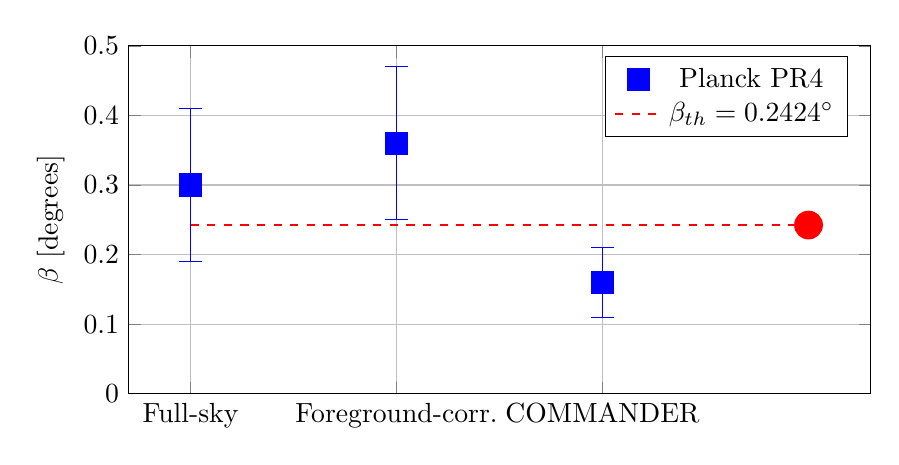
\begin{tikzpicture}
\begin{axis}[
    width=11cm, height=6cm,
    ylabel={$\beta$ [degrees]},
    symbolic x coords={Full-sky, Foreground-corr., COMMANDER, TFPT Theory},
    xtick=data,
    ymin=0, ymax=0.5,
    ytick={0, 0.1, 0.2, 0.3, 0.4, 0.5},
    grid=major,
    legend pos=north east,
]
    % Observations with error bars
    \addplot[
        only marks,
        mark=square*,
        mark size=4pt,
        blue,
        error bars/.cd,
        y dir=both, y explicit
    ] coordinates {(Full-sky,0.30) +- (0,0.11) (Foreground-corr.,0.36) +- (0,0.11) (COMMANDER,0.16) +- (0,0.05)};
    \addlegendentry{Planck PR4}
    
    % Theory line
    \addplot[thick, red, dashed, domain=0:4] coordinates {(Full-sky,0.2424) (Foreground-corr.,0.2424) (COMMANDER,0.2424) (TFPT Theory,0.2424)};
    \addlegendentry{$\beta_{\text{th}} = 0.2424^\circ$}
    
    % Theory point
    \addplot[only marks, mark=*, mark size=5pt, red] coordinates {(TFPT Theory,0.2424)};
\end{axis}
\end{tikzpicture}
\caption{Cosmic birefringence: TFPT prediction compared with Planck PR4 
measurements. Theory is within 0.5--1.7$\sigma$ of all observations.}
\label{fig:birefringence}
\end{figure}

%-----------------------------------------------------------------------------
\subsection{Two-Loop RG Fingerprints}
%-----------------------------------------------------------------------------

\begin{corollary}{RG Fingerprints}{RGfingerprints}
The TFPT invariants leave signatures in the RG flow of gauge couplings:
\begin{align}
    \alpha_3(1\,\text{PeV}) &\approx \phiz \quad 
        \text{(two-loop extrapolated: } 0.05244, \text{ expected: } 0.05317, 
        \text{ dev: } -1.38\%\text{)}\\
    \alpha_3(\mu_{\cthree}) &\approx \cthree \quad 
        \text{(two-loop extrapolated: } 0.0398, \text{ expected: } 0.0398, 
        \text{ dev: } 0.00\%\text{)}
\end{align}
These values are obtained by two-loop RG running from PDG boundary conditions at $M_Z$ using the declared PyR@TE model (checked by \texttt{two\_loop\_rg\_fingerprints} in \texttt{tfpt-suite/}; not direct measurements at the quoted scales). Here $\mu_{\cthree} \approx 2.16 \times 10^8$ GeV.
\end{corollary}

\begin{figure}[H]
\centering
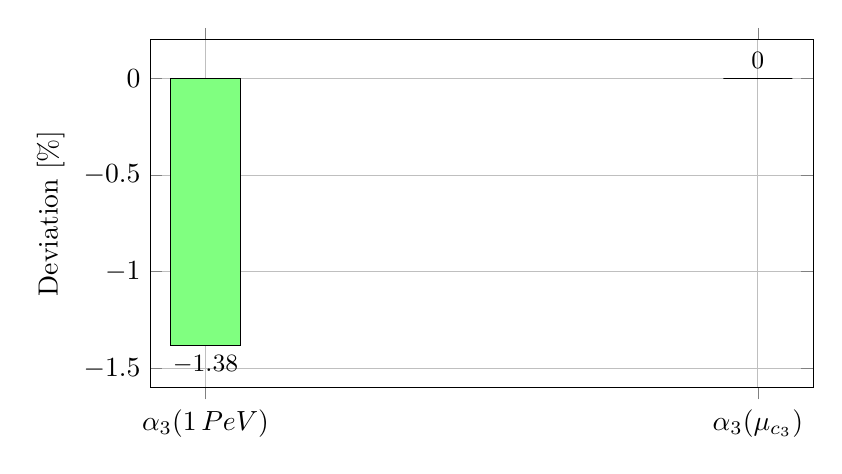
\begin{tikzpicture}
\begin{axis}[
    width=10cm, height=6cm,
    ybar,
    bar width=25pt,
    ylabel={Deviation [\%]},
    symbolic x coords={$\alpha_3(1\,\text{PeV})$, $\alpha_3(\mu_{c_3})$},
    xtick=data,
    ymin=-1.6, ymax=0.2,
    nodes near coords,
    nodes near coords align={vertical},
    every node near coord/.append style={font=\small},
    grid=major,
]
    \addplot[fill=green!50] coordinates 
        {($\alpha_3(1\,\text{PeV})$, -1.382) ($\alpha_3(\mu_{c_3})$, 0.000)};
\end{axis}
\end{tikzpicture}
\caption{Two-loop RG fingerprints: percent-level deviation from TFPT predictions at 1~PeV, and a constructed crossing for $\alpha_3(\mu_{\cthree})=\cthree$.}
\label{fig:twoloop}
\end{figure}

%=============================================================================
% PART II: STRUCTURAL EXTENSIONS
%=============================================================================
\vspace{1em}
\begin{center}
\rule{0.8\textwidth}{0.5pt}\\[0.5em]
{\Large\bfseries Part II: Structural Extensions}\\[0.3em]
{\small The following sections extend the core CFE framework. They are \\
testable structural postulates that do not affect the $\alpha$, $\beta$, \\
or RG fingerprint predictions established in Part I.}\\[0.5em]
\rule{0.8\textwidth}{0.5pt}
\end{center}
\vspace{1em}

%=============================================================================
\section{The E$_8$ Cascade and Block Constants}
%=============================================================================

%-----------------------------------------------------------------------------
\subsection{Nilpotent Orbit Structure}
%-----------------------------------------------------------------------------

\begin{definition}{E$_8$ Orbit Graph}{orbitgraph}
Let $\mathcal{N}(\mathfrak{e}_8)$ denote the set of nilpotent orbits of the 
exceptional Lie algebra $\mathfrak{e}_8$. For each orbit $\mathcal{O}$, define:
\begin{itemize}[leftmargin=1.5em, topsep=2pt, itemsep=1pt]
    \item $\dim(\mathcal{O})$: the dimension of the orbit as a variety
    \item $D(\mathcal{O}) = 248 - \dim(\mathcal{O})$: the ``centralizer dimension''
    \item $h(\mathcal{O})$: the height (sum of coefficients in weighted Dynkin diagram)
\end{itemize}
The \textbf{orbit graph} $G = (V, E)$ has vertices $V = \mathcal{N}(\mathfrak{e}_8)$ 
and directed edges $\mathcal{O} \to \mathcal{O}'$ iff:
\begin{enumerate}[leftmargin=1.5em, topsep=2pt, itemsep=1pt]
    \item $\mathcal{O}' \subset \overline{\mathcal{O}}$ (closure containment)
    \item $D(\mathcal{O}) - D(\mathcal{O}') = 2$ (minimal step)
\end{enumerate}
\end{definition}

\begin{theorem}{E$_8$ Chain Uniqueness}{chainunique}
Consider the closure ordering on $\mathcal{N}(\mathfrak{e}_8)$. There exists a 
\textbf{unique saturated chain} from the subregular orbit ($D = 58$) to the 
principal orbit ($D = 8$) satisfying:
\begin{enumerate}[leftmargin=1.5em, topsep=2pt, itemsep=1pt]
    \item All edges are cover relations with $\Delta D = 2$
    \item At each layer, the orbit of minimal height is selected
    \item The Levi structure is monotonically extended
\end{enumerate}
This chain has exactly 26 steps, yielding the sequence $D_n = 60 - 2n$ for $n = 1, \ldots, 26$.
\end{theorem}

\begin{proof}[Proof sketch]
The proof proceeds by explicit construction on the Hasse diagram of 
$\mathcal{N}(\mathfrak{e}_8)$:
\begin{enumerate}[leftmargin=1.5em, topsep=2pt, itemsep=1pt]
    \item \textbf{Layer structure:} Orbits are partitioned by $D$-value into 
        27 layers ($D \in \{60, 58, \ldots, 8\}$).
    \item \textbf{Cover relations:} For E$_8$, the cover relations are classified 
        by Bala--Carter labels. At each $D$-value, there may be multiple orbits, 
        but the height function provides a total order.
    \item \textbf{Uniqueness:} At each step $D \to D-2$, we select the unique 
        orbit that (a) is reachable from the current orbit via a cover relation, 
        and (b) has minimal height among all reachable candidates.
    \item \textbf{Verification:} The complete chain is given in Appendix~\ref{app:E8cert} 
        with explicit Bala--Carter labels.
\end{enumerate}
\end{proof}

%-----------------------------------------------------------------------------
